\chapter{February}

\section{Standard deviation} \index{Standard deviation}
\textbf{Standard deviation} $\sigma$ is defined as the square root of \textbf{variance}. That is,
\begin{align}
	\sigma(X) &= \sqrt{var(X)}
\end{align}
The definition for variance:
\begin{align}
var(X) = E[(X - \mu_X)^2]
\end{align}
The definition for \textbf{covariance}:
\begin{align}
cov(X,Y) = E[(X - \mu_X)(Y- \mu_Y)]
\end{align}
A property:
\begin{align}
	cov(X,X) = var(X) = \sigma(X)^2 
\end{align}
Definition for \textbf{correlation}:
\begin{align}
	\begin{split}
	\rho(X,Y) & = corr(X, Y) 		\\
			  & = \frac{cov(X,Y)}{\sigma_X \sigma_Y}
	\end{split}
\end{align}


\section{Determinant}\index{Determinant}
Today when I try to compute the determinant of the covariance matrix in the multivariate Gaussian, I come across the problem of overflow. In fact, I only
need to know the logarithm of the determinant. Therefore, I apply the following solution:
\begin{align}
	\begin{split}
	\log(\det A) &= \log(\Pi_{i=1}^{N} \lambda_i)  \\
				 & = \sum_{i=1}^{N} \log(\lambda_i)
	\end{split}
\end{align}

\section{Matplotlib}\index{Matplotlib}
Sample code to plot figures with Python:

\begin{minted}[frame=lines, framesep=2mm,]
	       {python}
x = np.linspace(-10, 4, 500, endpoint=True)
y = (3 * x + 12) / 4

fig = plt.figure()
fig.suptitle('Problem 3', fontsize=20, fontweight='bold')
ax = fig.add_subplot(111)
ax.plot(x, y)

ax.spines['right'].set_color('none')
ax.spines['top'].set_color('none')
ax.xaxis.set_ticks_position('bottom')
ax.spines['bottom'].set_position(('data',0))
ax.yaxis.set_ticks_position('left')
ax.spines['left'].set_position(('data',0))

plt.annotate(r'$(-4,0)$',
xy=(-4, 0), xycoords='data',
xytext=(-20, +60), textcoords='offset points', fontsize=16,
arrowprops=dict(arrowstyle="->", connectionstyle="arc3,rad=.2"))

plt.annotate(r'$(0,3)$',
xy=(0, 3), xycoords='data',
xytext=(+10, -30), textcoords='offset points', fontsize=16,
arrowprops=dict(arrowstyle="->", connectionstyle="arc3,rad=.2"))

plt.annotate(r'positive',
xy=(-6, 2), xycoords='data',
xytext=(+10, +30), textcoords='offset points', fontsize=16)

ax.set_xlabel("x")
ax.set_ylabel("y")

plt.savefig('3.png', dpi = 100)
plt.show()
\end{minted}

\section{Different types of machine learning methods:}
\begin{enumerate}
\item \textbf{Parametric methods}: a family of distributions that can be described using a finite 
number of paramters, such as \textit{GMM, Naive Bayes, SVM}.
\item \textbf{Non-parametric methods}: methods that are not based on parametrized families of
probability distributions, such as \textit{decision trees, KNN}. 
\end{enumerate}

The difference between parametric models and non-parametric models is that the former 
has a fixed number of parameters, while the latter grows the number of parameters with 
the amount of training data.
\begin{remark}
Note that the non-parametric model does not have no parameters: parameters are determined by the training data, not the model.
\end{remark}

Parametric models can also be categorized into \textbf{generative models} and 
\textbf{discriminative models}.
\begin{enumerate}
\item Generative models: Fit a probability distribution like a multivariate Gaussian to each class.
\item Approximate the boundaries between classes by simple functions.
\end{enumerate}

\section{Representation Learning}


\paragraph{Dimensionality Reduction and Denoising}
Given data in high-dimensional Euclidean space, project to a
low-dimensional linear subspace while retaining as much of the
signal as possible. 

\paragraph{Embedding and manifold learning}
Given data that lie in a non-Euclidean space, find an embedding into
Euclidean space that preserves as much of the geometry as possible.

\paragraph{Metric learning}
A metric $d$ should satisfy the following properties:
\begin{enumerate}
	\item $d(x, y) \geq 0$, non-negativity
	\item $d(x, y) = 0$ if and only if $x = y$
	\item $d(x, y) = d(y, x)$, symmetry
	\item $d(x, z) \leq d(x, y) + d(y, z)$, triangle inequality
\end{enumerate}

\section{Fast Nearest Neighbor Search}
\textbf{Locality sensitive hashing.}\hspace{0.2cm} Grouping points in space into \textit{buckets} based on some distance metric operating on the points. Points that are close to each other under the chosen metric are mapped to the same bucket with high probability.

\textbf{K-d tress.}\hspace{0.2cm} A space-partitioning data structure for organizing points in a k-dimensional space.

\begin{remark}
	Nearest neighbor is sensitive to noise.
\end{remark}

\section{Decision Trees}
\textbf{Node split.}\hspace{0.2cm} When to split a node, we need to decide which 
node to split. We have the following methods to measure the \textbf{uncertainty in prediction} $u(S)$:
\begin{itemize}
	\item \textit{Misclassification rate}: $min(p, 1-p)$, where $p$ is the fraction of positive points.
	\item \textit{Gini index}: $2p(1-p)$
	\item \textit{Entropy}: $-p\log p - (1-p)\log(1-p)$
\end{itemize}
We select the node split that can mostly reduce uncertainty (see Figure~\ref{fig:feb-dt-split}).
\begin{figure}[h]
	\centering{
		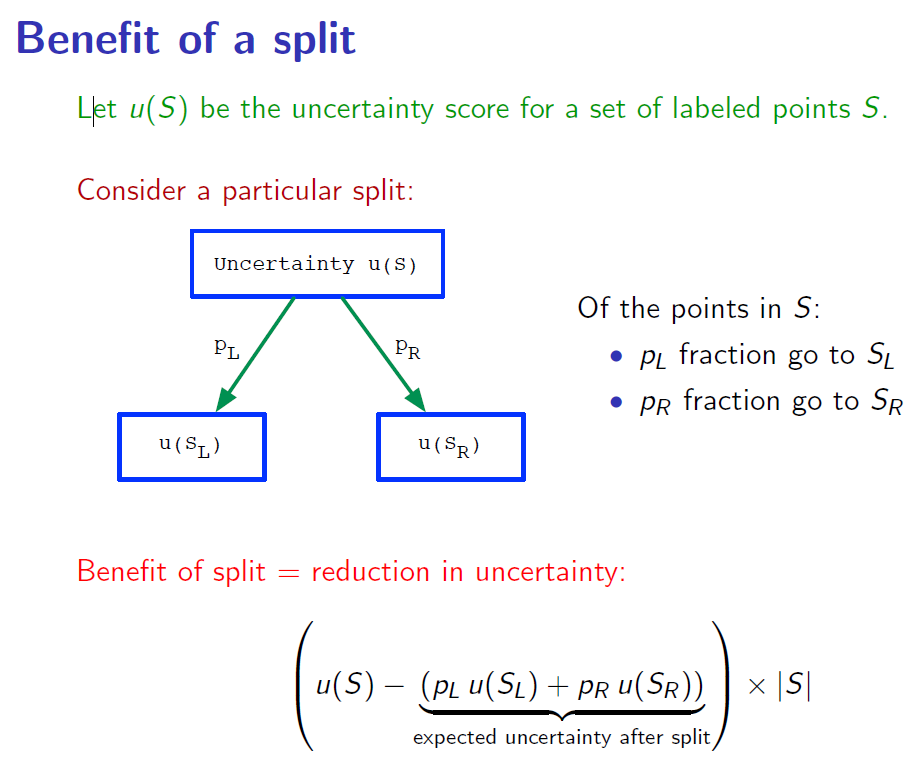
\includegraphics[width = 0.9\textwidth]{./images/feb/dt_split.PNG}
	}
	\label{fig:feb-dt-split}
	\caption{Benefit of a split.}
\end{figure} 


\textbf{When to stop?}\hspace{0.2cm} Keep splitting until leaves are pure. 

\textbf{Pruning.}\hspace{0.2cm} After split stops, we do pruning to avoid over-fitting. Consider all pairs of leave nodes,
any pair whose elimination yields a satisfactory (small)
increase in impurity is eliminated, and the common
antecedent node is declared as leaf node.

\section{Classification with generative models}

\textbf{Bayes-optimal prediction.}\hspace{0.2cm}
\begin{align}
	\begin{split}
	Pr(y= j | x) &= \frac{Pr(y= j) Pr(x|y=j)}{Pr(x)} \\
		&= \frac{\pi_j P_j(x)}{\sum_{i=1}^{k} \pi_i P_i(x)}
	\end{split}
\end{align}


\textbf{Laplace smoothing.}\hspace{0.2cm}
We want to estimate $p_{ji} = Pr(x_i = 1 | y=j)$. Then the maximum likelihood estimate of $p_{ji}$ is $p_{ij} = \frac{n_{ji}}{n_j}$, where $n_{ji}$ is the number of instances of class $j$ with $x_i = 1$, and $n_j$ is the number of 
instances of class $j$. 
\begin{remark}
This causes the problem if $n_{ji} = 0$. Instead, we use \textit{Laplace smoothing}: $p_{ji} = \frac{n_{ji} + 1}{n_j + 2}$
\end{remark} 


\textbf{Multinomial naive Bayes.}\hspace{0.2cm}
Classify document $x$ as $\argmax_j \pi_j \prod_{i=1}^{N} p_{ji} ^ {x_i}$.
To improve the performance, we may adopt the following heuristics:
\begin{itemize}
	\item Compensating for burstiness. Problem: once a word has appeared in a document, it has a much higher chance of appearing again.
	Solution: Instead of the number of occurrences $f$ of a word, use
	$\log(1 + f )$.
	
	\item Downweighting common words. Problem: common words can have a unduly large influence on classification. Solution: weight each word $w$ by \textit{inverse document frequency}:
	\[
		\log\frac{\# \text{docs}}{\#(\text{docs containing w})}
	\]
\end{itemize}

\section{Gaussian}
\textbf{Multivariate Gaussian.}\hspace{0.2cm} mean: $\mu \in R^p$. covariance $p\times p$
matrix $\sum$:
\begin{align}
\begin{split}
	p(x) &= \frac{1}{(2\pi)^{p/2} |\sum|^{1/2}} \exp(-\frac{1}{2} (x-\mu)^T \sum {}^{-1} (x-\mu))
\end{split}
\end{align}


\textbf{Spherical Gaussian.}\hspace{0.2cm} $\sum = diag(\sigma^2, ..., \sigma^2)$

Here we call it \textit{spherical Gaussian} because the contour of points with equal density is a sphere:
\begin{align}
\begin{split}
||x - \mu||^2 &= r^2
\end{split}
\end{align}

\begin{figure}[h]
\centering{
	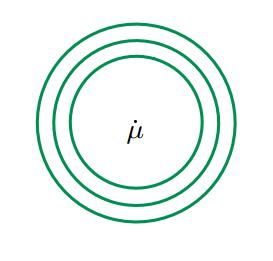
\includegraphics{./images/feb/sg.PNG}
}
\caption{The contour means that points on it have the same density. For spherical Gaussians, density at a point only depends on its distance from $\mu$.}
\end{figure}





\textbf{Diagonal Gaussian.}\hspace{0.2cm} $\sum = diag(\sigma_1^2, ..., \sigma_p^2)$

\begin{figure}[h]
	\centering{
		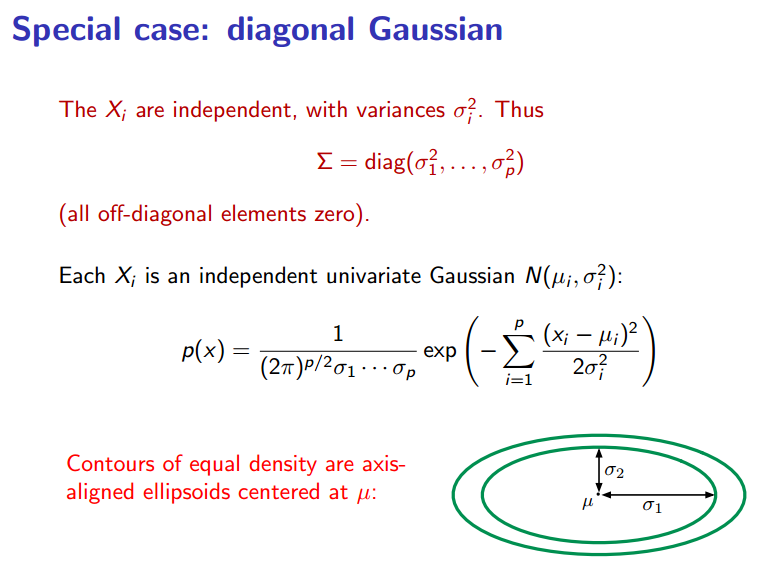
\includegraphics[width=0.9\textwidth]{./images/feb/dg.PNG}
	}
	\caption{Diagonal Gaussian: the contours are axis-aligned ellipsoids.}
\end{figure}

\myheader{General Gaussian .}

\begin{figure}[h]
	\centering{
		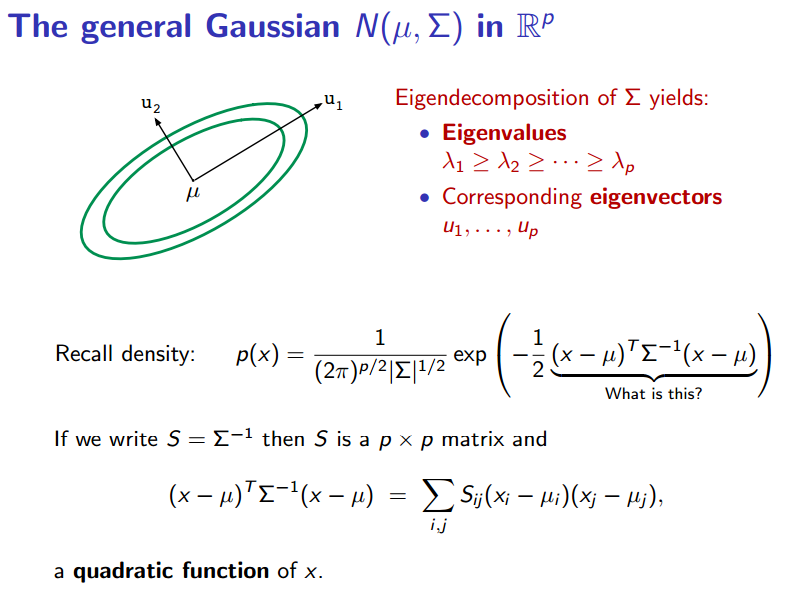
\includegraphics[width=0.9\textwidth]{./images/feb/gg.PNG}
	}
	\caption{General Gaussian: the contours are ellipsoids, with axis being the eigen-vectors
		of covariance matrix $\sum$.}
\end{figure}

\myheader{Binary classifications with Gaussians}
Suppose we have two Gaussians:
\begin{align}
\begin{split}
	P_1 &= N(\mu_1, \sum{}_1) \\
	P_2 &= N(\mu_2, \sum{}_2)
\end{split}
\end{align}

The classification boundary is:
\begin{align}
\begin{split}
	x^T M x + 2w^Tx & \geq \theta	\\
	\text{where } M & = \frac{1}{2}(\sum{}_2^{-1} - \sum{}_{1}^{-1}) \\
				w & = \sum{}_1^{-1} \mu_1 - \sum{}_{2}^{-1}\mu_2
\end{split}
\end{align}
\begin{remark}
	From this we know that, when $\sum_1 = \sum_2$, it has a linear decision boundary. Otherwise, it has quadratic boundary.
\end{remark}

\begin{remark}
	When calculate the inverse of covariance matrix $\sum$, to avoid the problem that $\sum$ 
	is singular, we need to regularize it: $\sum = \sum + \sigma^2 I$.
\end{remark}


\section{New commands in LaTex}
\begin{minted}[frame=lines, framesep=2mm,]
{cpp}
\newcommand{\plusbinomial}[3][2]{(#2 + #3)^#1}

To save some time when writing too many expressions 
with exponents is by defining a new command to make simpler:

\[ \plusbinomial{x}{y} \] -> $(x+y)^2$

And even the exponent can be changed

\[ \plusbinomial[4]{y}{y} \] -> $(y+y)^4$

\plusbinomial
This is the name of the new command.
[3]
The number of parameters the command will take, in this case 3.

[2]
Is the default value for the first parameter. This is what makes the first
 parameter optional, if not passed it will use this default value.

(#2 + #3)^#1
This is what the command does. In this case it will put the second and third
parameters in a "binomial format" to the power represented by the first
parameter.
\end{minted}


\section{OpenGL}

\subsection{Window Management in OpenGL .}
The OpenGL doesn't specify any API in order to create and manipulate windows. Modern windowing systems that support OpenGL include a sub-system that provides the binding between an OpenGL context and the windowing system. The library we use here is called \textit{OpenGL utility library}, or \textit{GLUT}. It provides a simplified API for window mangement as well 
as envent handling, IO control and few other services.

\myheader{State in OpenGL .}
Rendering is such a complex tas that it cannot be treated as a function call that receives a few paramters,
and correctly designed functions never receive a lot of parameters. You need to specify a lot of flags that affect
how rendering will take place. In addition, you would often want to keep the same piece of configuration across 
several rendering operations.  \textbf{That is why most of the configuration of rendering operations is done by setting
flags and values in the OpenGL state machine. After calling a state changing function that particular configuration
remains intact until the next call to the same function with a different value}.

\myheader{glutMainLoop .}
This call passes control to GLUT which now begins its own internal loop. In this loop it listens to events from 
the windowing system and passes them via callbacks that we configured.

\subsection{Hello dot}
\myheader{GLEW .} GLEW is short for \textbf{OpenGL Extension Wrangler Library}. GLEW helps you deal with
headache that can accompany the management of extensions in OpenGL.
			
\myheader{Vertex buffer objects .} VBOs are used to store vertices. They are the most efficient
way to load vertices into the GPU. The are buffers that can be stored in video memory and provide
the shortest access time to the GPU so they are definitely recommended.

\myheader{Rasterizer .} Rasterizer maps coordinates to screen space. And finally it draws the
primitives according to the topology which is specified in the draw call.




\section{Fisher's Linear Discriminant}
\myheader{What is Fisher LDA ?} Fisher LAD is a framework for linear classification without Gaussian assumptions. It is a linear classifier projects all data onto a direction $w$.

\begin{figure}[h]
	\centering{
		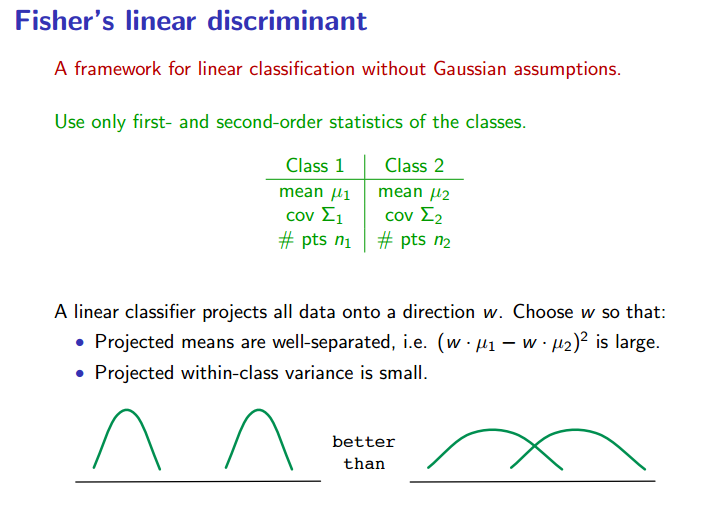
\includegraphics[width=0.45\textwidth]{./images/feb/LDA_1.PNG}
		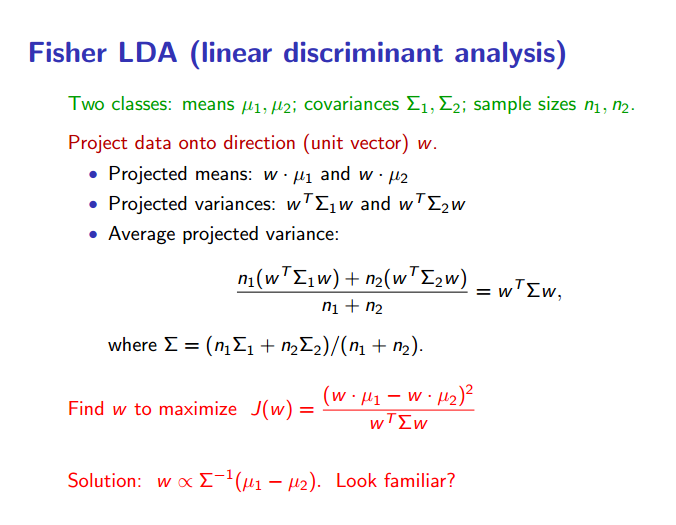
\includegraphics[width=0.45\textwidth]{./images/feb/LDA_2.PNG}	
	}
	\caption{Fisher LDA.}
\end{figure}

\section{Logistic Regression}
\myheader{Why Logistic Regression ?} See Figure~\ref{fig:logistic}.
\begin{figure}[t]
	\centering{
		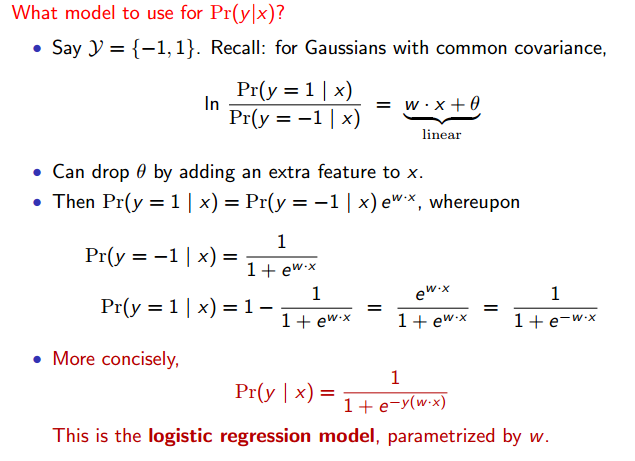
\includegraphics[width=0.45\textwidth]{./images/feb/logistic.PNG}
		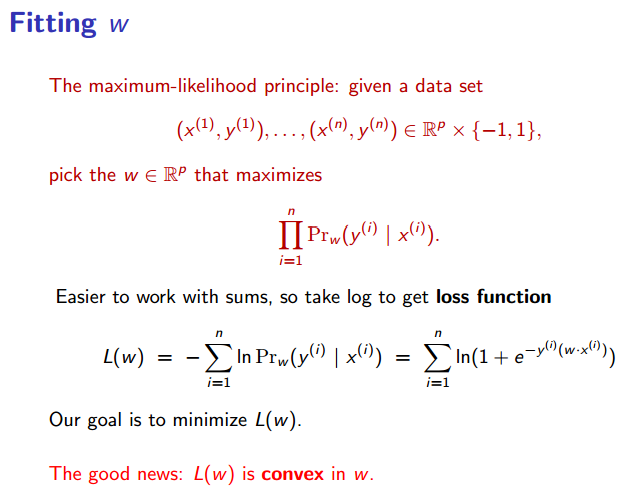
\includegraphics[width=0.45\textwidth]{./images/feb/logistic_1.PNG}	
	}
	\caption{Logistic regression.}
	\label{fig:logistic}
\end{figure}

\myheader{How to optimize $L(w)$ ?}
\begin{itemize}
\item \myheader{Gradient descent .} Gradient descent is a first-order optimization algorithm. To find a local minimum of a function using gradient descent, one takes steps proportional to the \textbf{negative} of the gradient (or of the approximate gradient) of the function at the current point. If instead one takes steps proportional to the positive of the gradient, one approaches a local maximum of that function; the procedure is then known as gradient ascent.

\item \myheader{Newton's method .} Newton's method is a method for finding successively better approximations to the roots (or zeroes) of a real-valued function: $f(x) = 0$. If the function satisfies the assumptions made in the derivation of the formula and the initial guess is close, then a better approximation $x_1$ is: $x_1 = x_0 - \frac{f(x_0)}{f'(x_0)}$.

To apply Newton's method for minimization and maximization problem, considering the fact that the derivative is zero at a minimum or maximum, so minima and maxima can be found by applying Newton's method to the derivative. The iteration becomes:
\[
x_{n+1} = x_n - \frac{f'(x_n)}{f''(x_n)}
\]
\end{itemize}

\myheader{How to determine step size ?} A method like Newton's method chooses a step, but the validity of that step only goes as far as the Newton quadratic model for the function really reflects the function. The idea of a line search is to use the direction of the chosen step, but to control the length, by solving a one-dimensional problem of minimizing
\[
\phi(\alpha) = f(\alpha p_k + x_k)
\]
where $p_k$ is is the search direction chosen from the position $x_k$.

\myheader{Backtracking line search .} 
First, fix a parameter $0 < \beta < 1, 0 < \alpha < 0.5$, then at each iteration, start with $t = 1$, and while 
\myequ{
	f(x - \nabla f(x)) &> f(x) -  \alpha t||\nabla f(x)||^2
}
update $t = \beta t$. 


\section{Matrix Calculus}
\myheader{First order derivatives}
\myequ{
	\frac{\partial AX}{\partial X} & = A^T \\
	\frac{\partial X^T a}{\partial X} &= a \\
	\frac{\partial a^T X b}{\partial X} &= ab^T \\
	\frac{\partial a^T X^T b}{\partial X} &= ba^T
}

\myheader{Jacobian matrix and Hessian matrix}
Jacobian matrix is the matrix of all \textbf{first-order partial derivatives} of a vector-valued function.
Hessian matrix is a square matrix of \textbf{second-order partial derivatives} of a scalar-valued function, or scalar field.

\section{Feature scaling}
Feature scaling is a method used to standardize the range of independent variables or features of data. In data processing, it is also known as data normalization and is generally performed during the data preprocessing step.

\myequ{
	x' &= \frac{x - \min(x)}{\max(x) - \min(x)}	
}

Since the range of values of raw data varies widely, in some machine learning algorithms, objective functions will not work properly without normalization. For example, the majority of classifiers calculate the distance between two points by the Euclidean distance. If one of the features has a broad range of values, the distance will be governed by this particular feature. Therefore, the range of all features should be normalized so that each feature contributes approximately proportionately to the final distance.

Another reason why feature scaling is applied is that gradient descent converges much faster with feature scaling than without it.























